% Created by tikzDevice version 0.7.0 on 2014-06-13 12:48:53
% !TEX encoding = UTF-8 Unicode
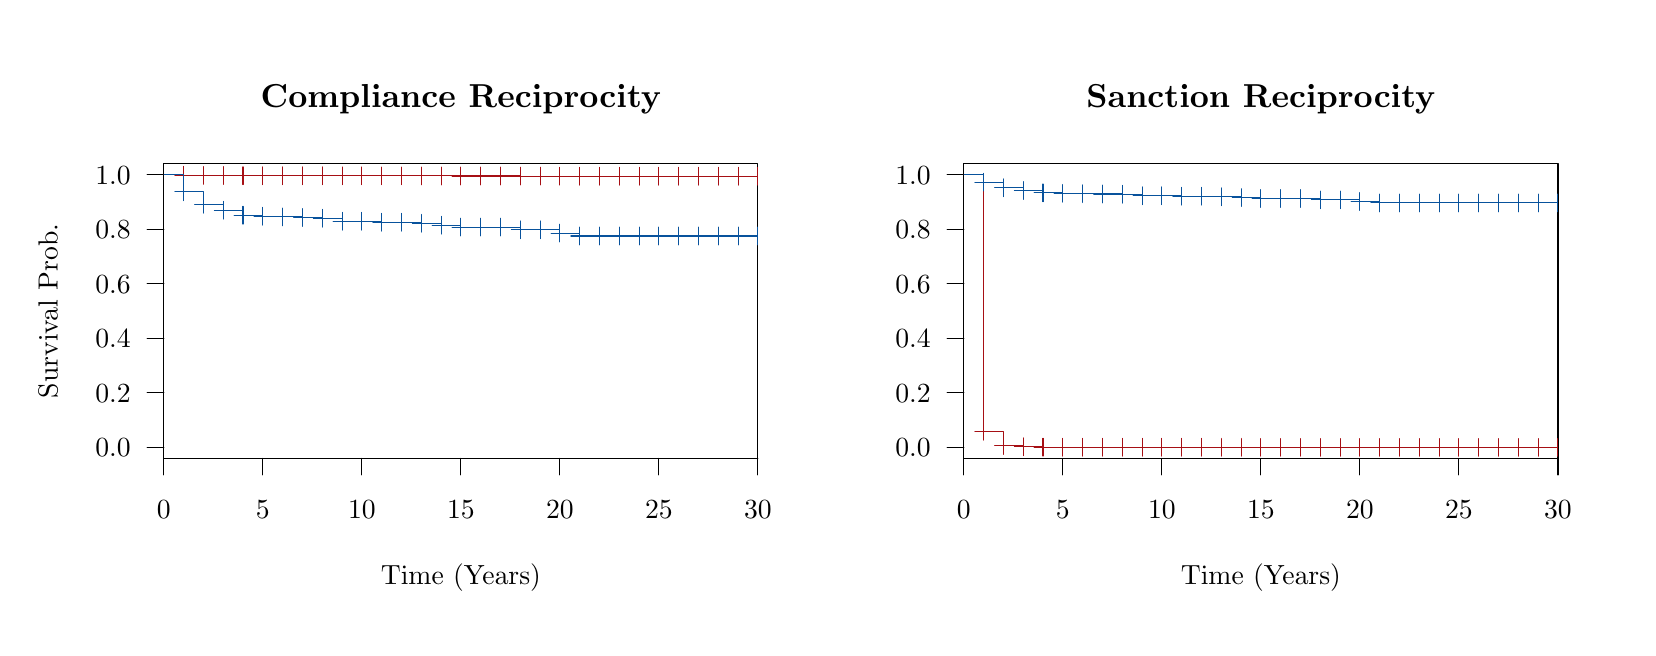
\begin{tikzpicture}[x=1pt,y=1pt]
\definecolor[named]{fillColor}{rgb}{1.00,1.00,1.00}
\path[use as bounding box,fill=fillColor,fill opacity=0.00] (0,0) rectangle (578.16,216.81);
\begin{scope}
\path[clip] (  0.00,  0.00) rectangle (578.16,216.81);
\definecolor[named]{drawColor}{rgb}{0.00,0.00,0.00}

\path[draw=drawColor,line width= 0.4pt,line join=round,line cap=round] ( 49.20, 61.20) -- (263.88, 61.20);

\path[draw=drawColor,line width= 0.4pt,line join=round,line cap=round] ( 49.20, 61.20) -- ( 49.20, 55.20);

\path[draw=drawColor,line width= 0.4pt,line join=round,line cap=round] ( 84.98, 61.20) -- ( 84.98, 55.20);

\path[draw=drawColor,line width= 0.4pt,line join=round,line cap=round] (120.76, 61.20) -- (120.76, 55.20);

\path[draw=drawColor,line width= 0.4pt,line join=round,line cap=round] (156.54, 61.20) -- (156.54, 55.20);

\path[draw=drawColor,line width= 0.4pt,line join=round,line cap=round] (192.32, 61.20) -- (192.32, 55.20);

\path[draw=drawColor,line width= 0.4pt,line join=round,line cap=round] (228.10, 61.20) -- (228.10, 55.20);

\path[draw=drawColor,line width= 0.4pt,line join=round,line cap=round] (263.88, 61.20) -- (263.88, 55.20);

\node[text=drawColor,anchor=base,inner sep=0pt, outer sep=0pt, scale=  1.00] at ( 49.20, 39.60) {0};

\node[text=drawColor,anchor=base,inner sep=0pt, outer sep=0pt, scale=  1.00] at ( 84.98, 39.60) {5};

\node[text=drawColor,anchor=base,inner sep=0pt, outer sep=0pt, scale=  1.00] at (120.76, 39.60) {10};

\node[text=drawColor,anchor=base,inner sep=0pt, outer sep=0pt, scale=  1.00] at (156.54, 39.60) {15};

\node[text=drawColor,anchor=base,inner sep=0pt, outer sep=0pt, scale=  1.00] at (192.32, 39.60) {20};

\node[text=drawColor,anchor=base,inner sep=0pt, outer sep=0pt, scale=  1.00] at (228.10, 39.60) {25};

\node[text=drawColor,anchor=base,inner sep=0pt, outer sep=0pt, scale=  1.00] at (263.88, 39.60) {30};

\path[draw=drawColor,line width= 0.4pt,line join=round,line cap=round] ( 49.20, 65.14) -- ( 49.20,163.67);

\path[draw=drawColor,line width= 0.4pt,line join=round,line cap=round] ( 49.20, 65.14) -- ( 43.20, 65.14);

\path[draw=drawColor,line width= 0.4pt,line join=round,line cap=round] ( 49.20, 84.85) -- ( 43.20, 84.85);

\path[draw=drawColor,line width= 0.4pt,line join=round,line cap=round] ( 49.20,104.55) -- ( 43.20,104.55);

\path[draw=drawColor,line width= 0.4pt,line join=round,line cap=round] ( 49.20,124.26) -- ( 43.20,124.26);

\path[draw=drawColor,line width= 0.4pt,line join=round,line cap=round] ( 49.20,143.96) -- ( 43.20,143.96);

\path[draw=drawColor,line width= 0.4pt,line join=round,line cap=round] ( 49.20,163.67) -- ( 43.20,163.67);

\node[text=drawColor,anchor=base east,inner sep=0pt, outer sep=0pt, scale=  1.00] at ( 37.20, 61.70) {0.0};

\node[text=drawColor,anchor=base east,inner sep=0pt, outer sep=0pt, scale=  1.00] at ( 37.20, 81.40) {0.2};

\node[text=drawColor,anchor=base east,inner sep=0pt, outer sep=0pt, scale=  1.00] at ( 37.20,101.11) {0.4};

\node[text=drawColor,anchor=base east,inner sep=0pt, outer sep=0pt, scale=  1.00] at ( 37.20,120.81) {0.6};

\node[text=drawColor,anchor=base east,inner sep=0pt, outer sep=0pt, scale=  1.00] at ( 37.20,140.52) {0.8};

\node[text=drawColor,anchor=base east,inner sep=0pt, outer sep=0pt, scale=  1.00] at ( 37.20,160.23) {1.0};

\path[draw=drawColor,line width= 0.4pt,line join=round,line cap=round] ( 49.20, 61.20) --
	(263.88, 61.20) --
	(263.88,167.61) --
	( 49.20,167.61) --
	( 49.20, 61.20);
\end{scope}
\begin{scope}
\path[clip] (  0.00,  0.00) rectangle (289.08,216.81);
\definecolor[named]{drawColor}{rgb}{0.00,0.00,0.00}

\node[text=drawColor,anchor=base,inner sep=0pt, outer sep=0pt, scale=  1.20] at (156.54,188.07) {\bfseries Compliance Reciprocity};
\end{scope}
\begin{scope}
\path[clip] ( 49.20, 61.20) rectangle (263.88,167.61);
\definecolor[named]{drawColor}{rgb}{0.65,0.06,0.08}

\path[draw=drawColor,line width= 0.4pt,line join=round,line cap=round] ( 49.20,163.67) --
	( 56.36,163.67) --
	( 56.36,163.53) --
	( 63.51,163.53) --
	( 63.51,163.42) --
	( 70.67,163.42) --
	( 70.67,163.37) --
	( 77.82,163.37) --
	( 77.82,163.32) --
	( 84.98,163.32) --
	( 84.98,163.31) --
	( 92.14,163.31) --
	( 92.14,163.31) --
	( 99.29,163.31) --
	( 99.29,163.30) --
	(106.45,163.30) --
	(106.45,163.29) --
	(113.60,163.29) --
	(113.60,163.26) --
	(127.92,163.26) --
	(127.92,163.26) --
	(142.23,163.26) --
	(142.23,163.24) --
	(149.38,163.24) --
	(149.38,163.23) --
	(156.54,163.23) --
	(156.54,163.21) --
	(178.01,163.21) --
	(178.01,163.18) --
	(192.32,163.18) --
	(192.32,163.15) --
	(199.48,163.15) --
	(199.48,163.12) --
	(464.25,163.12) --
	(464.25,163.12);

\path[draw=drawColor,line width= 0.4pt,line join=round,line cap=round] ( 53.17,163.53) -- ( 59.54,163.53);

\path[draw=drawColor,line width= 0.4pt,line join=round,line cap=round] ( 56.36,160.35) -- ( 56.36,166.71);

\path[draw=drawColor,line width= 0.4pt,line join=round,line cap=round] ( 60.33,163.42) -- ( 66.69,163.42);

\path[draw=drawColor,line width= 0.4pt,line join=round,line cap=round] ( 63.51,160.24) -- ( 63.51,166.60);

\path[draw=drawColor,line width= 0.4pt,line join=round,line cap=round] ( 67.49,163.37) -- ( 73.85,163.37);

\path[draw=drawColor,line width= 0.4pt,line join=round,line cap=round] ( 70.67,160.19) -- ( 70.67,166.55);

\path[draw=drawColor,line width= 0.4pt,line join=round,line cap=round] ( 74.64,163.32) -- ( 81.01,163.32);

\path[draw=drawColor,line width= 0.4pt,line join=round,line cap=round] ( 77.82,160.14) -- ( 77.82,166.50);

\path[draw=drawColor,line width= 0.4pt,line join=round,line cap=round] ( 81.80,163.31) -- ( 88.16,163.31);

\path[draw=drawColor,line width= 0.4pt,line join=round,line cap=round] ( 84.98,160.13) -- ( 84.98,166.49);

\path[draw=drawColor,line width= 0.4pt,line join=round,line cap=round] ( 88.95,163.31) -- ( 95.32,163.31);

\path[draw=drawColor,line width= 0.4pt,line join=round,line cap=round] ( 92.14,160.12) -- ( 92.14,166.49);

\path[draw=drawColor,line width= 0.4pt,line join=round,line cap=round] ( 96.11,163.30) -- (102.47,163.30);

\path[draw=drawColor,line width= 0.4pt,line join=round,line cap=round] ( 99.29,160.12) -- ( 99.29,166.48);

\path[draw=drawColor,line width= 0.4pt,line join=round,line cap=round] (103.27,163.29) -- (109.63,163.29);

\path[draw=drawColor,line width= 0.4pt,line join=round,line cap=round] (106.45,160.11) -- (106.45,166.47);

\path[draw=drawColor,line width= 0.4pt,line join=round,line cap=round] (110.42,163.26) -- (116.79,163.26);

\path[draw=drawColor,line width= 0.4pt,line join=round,line cap=round] (113.60,160.08) -- (113.60,166.45);

\path[draw=drawColor,line width= 0.4pt,line join=round,line cap=round] (117.58,163.26) -- (123.94,163.26);

\path[draw=drawColor,line width= 0.4pt,line join=round,line cap=round] (120.76,160.08) -- (120.76,166.45);

\path[draw=drawColor,line width= 0.4pt,line join=round,line cap=round] (124.73,163.26) -- (131.10,163.26);

\path[draw=drawColor,line width= 0.4pt,line join=round,line cap=round] (127.92,160.07) -- (127.92,166.44);

\path[draw=drawColor,line width= 0.4pt,line join=round,line cap=round] (131.89,163.26) -- (138.25,163.26);

\path[draw=drawColor,line width= 0.4pt,line join=round,line cap=round] (135.07,160.07) -- (135.07,166.44);

\path[draw=drawColor,line width= 0.4pt,line join=round,line cap=round] (139.05,163.24) -- (145.41,163.24);

\path[draw=drawColor,line width= 0.4pt,line join=round,line cap=round] (142.23,160.06) -- (142.23,166.43);

\path[draw=drawColor,line width= 0.4pt,line join=round,line cap=round] (146.20,163.23) -- (152.57,163.23);

\path[draw=drawColor,line width= 0.4pt,line join=round,line cap=round] (149.38,160.05) -- (149.38,166.41);

\path[draw=drawColor,line width= 0.4pt,line join=round,line cap=round] (153.36,163.21) -- (159.72,163.21);

\path[draw=drawColor,line width= 0.4pt,line join=round,line cap=round] (156.54,160.03) -- (156.54,166.39);

\path[draw=drawColor,line width= 0.4pt,line join=round,line cap=round] (160.51,163.21) -- (166.88,163.21);

\path[draw=drawColor,line width= 0.4pt,line join=round,line cap=round] (163.70,160.03) -- (163.70,166.39);

\path[draw=drawColor,line width= 0.4pt,line join=round,line cap=round] (167.67,163.21) -- (174.03,163.21);

\path[draw=drawColor,line width= 0.4pt,line join=round,line cap=round] (170.85,160.03) -- (170.85,166.39);

\path[draw=drawColor,line width= 0.4pt,line join=round,line cap=round] (174.83,163.18) -- (181.19,163.18);

\path[draw=drawColor,line width= 0.4pt,line join=round,line cap=round] (178.01,160.00) -- (178.01,166.36);

\path[draw=drawColor,line width= 0.4pt,line join=round,line cap=round] (181.98,163.18) -- (188.35,163.18);

\path[draw=drawColor,line width= 0.4pt,line join=round,line cap=round] (185.16,160.00) -- (185.16,166.36);

\path[draw=drawColor,line width= 0.4pt,line join=round,line cap=round] (189.14,163.15) -- (195.50,163.15);

\path[draw=drawColor,line width= 0.4pt,line join=round,line cap=round] (192.32,159.97) -- (192.32,166.33);

\path[draw=drawColor,line width= 0.4pt,line join=round,line cap=round] (196.29,163.12) -- (202.66,163.12);

\path[draw=drawColor,line width= 0.4pt,line join=round,line cap=round] (199.48,159.94) -- (199.48,166.30);

\path[draw=drawColor,line width= 0.4pt,line join=round,line cap=round] (203.45,163.12) -- (209.81,163.12);

\path[draw=drawColor,line width= 0.4pt,line join=round,line cap=round] (206.63,159.94) -- (206.63,166.30);

\path[draw=drawColor,line width= 0.4pt,line join=round,line cap=round] (210.61,163.12) -- (216.97,163.12);

\path[draw=drawColor,line width= 0.4pt,line join=round,line cap=round] (213.79,159.94) -- (213.79,166.30);

\path[draw=drawColor,line width= 0.4pt,line join=round,line cap=round] (217.76,163.12) -- (224.13,163.12);

\path[draw=drawColor,line width= 0.4pt,line join=round,line cap=round] (220.94,159.94) -- (220.94,166.30);

\path[draw=drawColor,line width= 0.4pt,line join=round,line cap=round] (224.92,163.12) -- (231.28,163.12);

\path[draw=drawColor,line width= 0.4pt,line join=round,line cap=round] (228.10,159.94) -- (228.10,166.30);

\path[draw=drawColor,line width= 0.4pt,line join=round,line cap=round] (232.07,163.12) -- (238.44,163.12);

\path[draw=drawColor,line width= 0.4pt,line join=round,line cap=round] (235.26,159.94) -- (235.26,166.30);

\path[draw=drawColor,line width= 0.4pt,line join=round,line cap=round] (239.23,163.12) -- (245.59,163.12);

\path[draw=drawColor,line width= 0.4pt,line join=round,line cap=round] (242.41,159.94) -- (242.41,166.30);

\path[draw=drawColor,line width= 0.4pt,line join=round,line cap=round] (246.39,163.12) -- (252.75,163.12);

\path[draw=drawColor,line width= 0.4pt,line join=round,line cap=round] (249.57,159.94) -- (249.57,166.30);

\path[draw=drawColor,line width= 0.4pt,line join=round,line cap=round] (253.54,163.12) -- (259.91,163.12);

\path[draw=drawColor,line width= 0.4pt,line join=round,line cap=round] (256.72,159.94) -- (256.72,166.30);

\path[draw=drawColor,line width= 0.4pt,line join=round,line cap=round] (260.70,163.12) -- (267.06,163.12);

\path[draw=drawColor,line width= 0.4pt,line join=round,line cap=round] (263.88,159.94) -- (263.88,166.30);

\path[draw=drawColor,line width= 0.4pt,line join=round,line cap=round] (267.85,163.12) -- (274.22,163.12);

\path[draw=drawColor,line width= 0.4pt,line join=round,line cap=round] (271.04,159.94) -- (271.04,166.30);

\path[draw=drawColor,line width= 0.4pt,line join=round,line cap=round] (275.01,163.12) -- (281.37,163.12);

\path[draw=drawColor,line width= 0.4pt,line join=round,line cap=round] (278.19,159.94) -- (278.19,166.30);

\path[draw=drawColor,line width= 0.4pt,line join=round,line cap=round] (282.17,163.12) -- (288.53,163.12);

\path[draw=drawColor,line width= 0.4pt,line join=round,line cap=round] (285.35,159.94) -- (285.35,166.30);

\path[draw=drawColor,line width= 0.4pt,line join=round,line cap=round] (289.32,163.12) -- (295.69,163.12);

\path[draw=drawColor,line width= 0.4pt,line join=round,line cap=round] (292.50,159.94) -- (292.50,166.30);

\path[draw=drawColor,line width= 0.4pt,line join=round,line cap=round] (296.48,163.12) -- (302.84,163.12);

\path[draw=drawColor,line width= 0.4pt,line join=round,line cap=round] (299.66,159.94) -- (299.66,166.30);

\path[draw=drawColor,line width= 0.4pt,line join=round,line cap=round] (303.63,163.12) -- (310.00,163.12);

\path[draw=drawColor,line width= 0.4pt,line join=round,line cap=round] (306.82,159.94) -- (306.82,166.30);

\path[draw=drawColor,line width= 0.4pt,line join=round,line cap=round] (310.79,163.12) -- (317.15,163.12);

\path[draw=drawColor,line width= 0.4pt,line join=round,line cap=round] (313.97,159.94) -- (313.97,166.30);

\path[draw=drawColor,line width= 0.4pt,line join=round,line cap=round] (317.95,163.12) -- (324.31,163.12);

\path[draw=drawColor,line width= 0.4pt,line join=round,line cap=round] (321.13,159.94) -- (321.13,166.30);

\path[draw=drawColor,line width= 0.4pt,line join=round,line cap=round] (325.10,163.12) -- (331.47,163.12);

\path[draw=drawColor,line width= 0.4pt,line join=round,line cap=round] (328.28,159.94) -- (328.28,166.30);

\path[draw=drawColor,line width= 0.4pt,line join=round,line cap=round] (332.26,163.12) -- (338.62,163.12);

\path[draw=drawColor,line width= 0.4pt,line join=round,line cap=round] (335.44,159.94) -- (335.44,166.30);

\path[draw=drawColor,line width= 0.4pt,line join=round,line cap=round] (339.41,163.12) -- (345.78,163.12);

\path[draw=drawColor,line width= 0.4pt,line join=round,line cap=round] (342.60,159.94) -- (342.60,166.30);

\path[draw=drawColor,line width= 0.4pt,line join=round,line cap=round] (346.57,163.12) -- (352.93,163.12);

\path[draw=drawColor,line width= 0.4pt,line join=round,line cap=round] (349.75,159.94) -- (349.75,166.30);

\path[draw=drawColor,line width= 0.4pt,line join=round,line cap=round] (353.73,163.12) -- (360.09,163.12);

\path[draw=drawColor,line width= 0.4pt,line join=round,line cap=round] (356.91,159.94) -- (356.91,166.30);

\path[draw=drawColor,line width= 0.4pt,line join=round,line cap=round] (360.88,163.12) -- (367.25,163.12);

\path[draw=drawColor,line width= 0.4pt,line join=round,line cap=round] (364.06,159.94) -- (364.06,166.30);

\path[draw=drawColor,line width= 0.4pt,line join=round,line cap=round] (368.04,163.12) -- (374.40,163.12);

\path[draw=drawColor,line width= 0.4pt,line join=round,line cap=round] (371.22,159.94) -- (371.22,166.30);

\path[draw=drawColor,line width= 0.4pt,line join=round,line cap=round] (375.19,163.12) -- (381.56,163.12);

\path[draw=drawColor,line width= 0.4pt,line join=round,line cap=round] (378.38,159.94) -- (378.38,166.30);

\path[draw=drawColor,line width= 0.4pt,line join=round,line cap=round] (382.35,163.12) -- (388.71,163.12);

\path[draw=drawColor,line width= 0.4pt,line join=round,line cap=round] (385.53,159.94) -- (385.53,166.30);

\path[draw=drawColor,line width= 0.4pt,line join=round,line cap=round] (389.51,163.12) -- (395.87,163.12);

\path[draw=drawColor,line width= 0.4pt,line join=round,line cap=round] (392.69,159.94) -- (392.69,166.30);

\path[draw=drawColor,line width= 0.4pt,line join=round,line cap=round] (396.66,163.12) -- (403.03,163.12);

\path[draw=drawColor,line width= 0.4pt,line join=round,line cap=round] (399.84,159.94) -- (399.84,166.30);

\path[draw=drawColor,line width= 0.4pt,line join=round,line cap=round] (403.82,163.12) -- (410.18,163.12);

\path[draw=drawColor,line width= 0.4pt,line join=round,line cap=round] (407.00,159.94) -- (407.00,166.30);

\path[draw=drawColor,line width= 0.4pt,line join=round,line cap=round] (410.97,163.12) -- (417.34,163.12);

\path[draw=drawColor,line width= 0.4pt,line join=round,line cap=round] (414.16,159.94) -- (414.16,166.30);

\path[draw=drawColor,line width= 0.4pt,line join=round,line cap=round] (418.13,163.12) -- (424.49,163.12);

\path[draw=drawColor,line width= 0.4pt,line join=round,line cap=round] (421.31,159.94) -- (421.31,166.30);

\path[draw=drawColor,line width= 0.4pt,line join=round,line cap=round] (425.29,163.12) -- (431.65,163.12);

\path[draw=drawColor,line width= 0.4pt,line join=round,line cap=round] (428.47,159.94) -- (428.47,166.30);

\path[draw=drawColor,line width= 0.4pt,line join=round,line cap=round] (432.44,163.12) -- (438.81,163.12);

\path[draw=drawColor,line width= 0.4pt,line join=round,line cap=round] (435.62,159.94) -- (435.62,166.30);

\path[draw=drawColor,line width= 0.4pt,line join=round,line cap=round] (439.60,163.12) -- (445.96,163.12);

\path[draw=drawColor,line width= 0.4pt,line join=round,line cap=round] (442.78,159.94) -- (442.78,166.30);

\path[draw=drawColor,line width= 0.4pt,line join=round,line cap=round] (446.75,163.12) -- (453.12,163.12);

\path[draw=drawColor,line width= 0.4pt,line join=round,line cap=round] (449.94,159.94) -- (449.94,166.30);

\path[draw=drawColor,line width= 0.4pt,line join=round,line cap=round] (453.91,163.12) -- (460.27,163.12);

\path[draw=drawColor,line width= 0.4pt,line join=round,line cap=round] (457.09,159.94) -- (457.09,166.30);

\path[draw=drawColor,line width= 0.4pt,line join=round,line cap=round] (461.07,163.12) -- (467.43,163.12);

\path[draw=drawColor,line width= 0.4pt,line join=round,line cap=round] (464.25,159.94) -- (464.25,166.30);
\definecolor[named]{drawColor}{rgb}{0.03,0.32,0.61}

\path[draw=drawColor,line width= 0.4pt,line join=round,line cap=round] ( 49.20,163.67) --
	( 56.36,163.67) --
	( 56.36,157.53) --
	( 63.51,157.53) --
	( 63.51,153.02) --
	( 70.67,153.02) --
	( 70.67,150.86) --
	( 77.82,150.86) --
	( 77.82,149.05) --
	( 84.98,149.05) --
	( 84.98,148.67) --
	( 92.14,148.67) --
	( 92.14,148.43) --
	( 99.29,148.43) --
	( 99.29,148.20) --
	(106.45,148.20) --
	(106.45,147.94) --
	(113.60,147.94) --
	(113.60,146.85) --
	(127.92,146.85) --
	(127.92,146.52) --
	(142.23,146.52) --
	(142.23,146.10) --
	(149.38,146.10) --
	(149.38,145.44) --
	(156.54,145.44) --
	(156.54,144.74) --
	(178.01,144.74) --
	(178.01,143.76) --
	(192.32,143.76) --
	(192.32,142.58) --
	(199.48,142.58) --
	(199.48,141.51) --
	(464.25,141.51) --
	(464.25,141.51);

\path[draw=drawColor,line width= 0.4pt,line join=round,line cap=round] ( 53.17,157.53) -- ( 59.54,157.53);

\path[draw=drawColor,line width= 0.4pt,line join=round,line cap=round] ( 56.36,154.34) -- ( 56.36,160.71);

\path[draw=drawColor,line width= 0.4pt,line join=round,line cap=round] ( 60.33,153.02) -- ( 66.69,153.02);

\path[draw=drawColor,line width= 0.4pt,line join=round,line cap=round] ( 63.51,149.84) -- ( 63.51,156.20);

\path[draw=drawColor,line width= 0.4pt,line join=round,line cap=round] ( 67.49,150.86) -- ( 73.85,150.86);

\path[draw=drawColor,line width= 0.4pt,line join=round,line cap=round] ( 70.67,147.68) -- ( 70.67,154.04);

\path[draw=drawColor,line width= 0.4pt,line join=round,line cap=round] ( 74.64,149.05) -- ( 81.01,149.05);

\path[draw=drawColor,line width= 0.4pt,line join=round,line cap=round] ( 77.82,145.87) -- ( 77.82,152.23);

\path[draw=drawColor,line width= 0.4pt,line join=round,line cap=round] ( 81.80,148.67) -- ( 88.16,148.67);

\path[draw=drawColor,line width= 0.4pt,line join=round,line cap=round] ( 84.98,145.49) -- ( 84.98,151.85);

\path[draw=drawColor,line width= 0.4pt,line join=round,line cap=round] ( 88.95,148.43) -- ( 95.32,148.43);

\path[draw=drawColor,line width= 0.4pt,line join=round,line cap=round] ( 92.14,145.25) -- ( 92.14,151.61);

\path[draw=drawColor,line width= 0.4pt,line join=round,line cap=round] ( 96.11,148.20) -- (102.47,148.20);

\path[draw=drawColor,line width= 0.4pt,line join=round,line cap=round] ( 99.29,145.02) -- ( 99.29,151.39);

\path[draw=drawColor,line width= 0.4pt,line join=round,line cap=round] (103.27,147.94) -- (109.63,147.94);

\path[draw=drawColor,line width= 0.4pt,line join=round,line cap=round] (106.45,144.75) -- (106.45,151.12);

\path[draw=drawColor,line width= 0.4pt,line join=round,line cap=round] (110.42,146.85) -- (116.79,146.85);

\path[draw=drawColor,line width= 0.4pt,line join=round,line cap=round] (113.60,143.66) -- (113.60,150.03);

\path[draw=drawColor,line width= 0.4pt,line join=round,line cap=round] (117.58,146.85) -- (123.94,146.85);

\path[draw=drawColor,line width= 0.4pt,line join=round,line cap=round] (120.76,143.66) -- (120.76,150.03);

\path[draw=drawColor,line width= 0.4pt,line join=round,line cap=round] (124.73,146.52) -- (131.10,146.52);

\path[draw=drawColor,line width= 0.4pt,line join=round,line cap=round] (127.92,143.34) -- (127.92,149.70);

\path[draw=drawColor,line width= 0.4pt,line join=round,line cap=round] (131.89,146.52) -- (138.25,146.52);

\path[draw=drawColor,line width= 0.4pt,line join=round,line cap=round] (135.07,143.34) -- (135.07,149.70);

\path[draw=drawColor,line width= 0.4pt,line join=round,line cap=round] (139.05,146.10) -- (145.41,146.10);

\path[draw=drawColor,line width= 0.4pt,line join=round,line cap=round] (142.23,142.92) -- (142.23,149.29);

\path[draw=drawColor,line width= 0.4pt,line join=round,line cap=round] (146.20,145.44) -- (152.57,145.44);

\path[draw=drawColor,line width= 0.4pt,line join=round,line cap=round] (149.38,142.26) -- (149.38,148.62);

\path[draw=drawColor,line width= 0.4pt,line join=round,line cap=round] (153.36,144.74) -- (159.72,144.74);

\path[draw=drawColor,line width= 0.4pt,line join=round,line cap=round] (156.54,141.56) -- (156.54,147.93);

\path[draw=drawColor,line width= 0.4pt,line join=round,line cap=round] (160.51,144.74) -- (166.88,144.74);

\path[draw=drawColor,line width= 0.4pt,line join=round,line cap=round] (163.70,141.56) -- (163.70,147.93);

\path[draw=drawColor,line width= 0.4pt,line join=round,line cap=round] (167.67,144.74) -- (174.03,144.74);

\path[draw=drawColor,line width= 0.4pt,line join=round,line cap=round] (170.85,141.56) -- (170.85,147.93);

\path[draw=drawColor,line width= 0.4pt,line join=round,line cap=round] (174.83,143.76) -- (181.19,143.76);

\path[draw=drawColor,line width= 0.4pt,line join=round,line cap=round] (178.01,140.57) -- (178.01,146.94);

\path[draw=drawColor,line width= 0.4pt,line join=round,line cap=round] (181.98,143.76) -- (188.35,143.76);

\path[draw=drawColor,line width= 0.4pt,line join=round,line cap=round] (185.16,140.57) -- (185.16,146.94);

\path[draw=drawColor,line width= 0.4pt,line join=round,line cap=round] (189.14,142.58) -- (195.50,142.58);

\path[draw=drawColor,line width= 0.4pt,line join=round,line cap=round] (192.32,139.40) -- (192.32,145.76);

\path[draw=drawColor,line width= 0.4pt,line join=round,line cap=round] (196.29,141.51) -- (202.66,141.51);

\path[draw=drawColor,line width= 0.4pt,line join=round,line cap=round] (199.48,138.33) -- (199.48,144.69);

\path[draw=drawColor,line width= 0.4pt,line join=round,line cap=round] (203.45,141.51) -- (209.81,141.51);

\path[draw=drawColor,line width= 0.4pt,line join=round,line cap=round] (206.63,138.33) -- (206.63,144.69);

\path[draw=drawColor,line width= 0.4pt,line join=round,line cap=round] (210.61,141.51) -- (216.97,141.51);

\path[draw=drawColor,line width= 0.4pt,line join=round,line cap=round] (213.79,138.33) -- (213.79,144.69);

\path[draw=drawColor,line width= 0.4pt,line join=round,line cap=round] (217.76,141.51) -- (224.13,141.51);

\path[draw=drawColor,line width= 0.4pt,line join=round,line cap=round] (220.94,138.33) -- (220.94,144.69);

\path[draw=drawColor,line width= 0.4pt,line join=round,line cap=round] (224.92,141.51) -- (231.28,141.51);

\path[draw=drawColor,line width= 0.4pt,line join=round,line cap=round] (228.10,138.33) -- (228.10,144.69);

\path[draw=drawColor,line width= 0.4pt,line join=round,line cap=round] (232.07,141.51) -- (238.44,141.51);

\path[draw=drawColor,line width= 0.4pt,line join=round,line cap=round] (235.26,138.33) -- (235.26,144.69);

\path[draw=drawColor,line width= 0.4pt,line join=round,line cap=round] (239.23,141.51) -- (245.59,141.51);

\path[draw=drawColor,line width= 0.4pt,line join=round,line cap=round] (242.41,138.33) -- (242.41,144.69);

\path[draw=drawColor,line width= 0.4pt,line join=round,line cap=round] (246.39,141.51) -- (252.75,141.51);

\path[draw=drawColor,line width= 0.4pt,line join=round,line cap=round] (249.57,138.33) -- (249.57,144.69);

\path[draw=drawColor,line width= 0.4pt,line join=round,line cap=round] (253.54,141.51) -- (259.91,141.51);

\path[draw=drawColor,line width= 0.4pt,line join=round,line cap=round] (256.72,138.33) -- (256.72,144.69);

\path[draw=drawColor,line width= 0.4pt,line join=round,line cap=round] (260.70,141.51) -- (267.06,141.51);

\path[draw=drawColor,line width= 0.4pt,line join=round,line cap=round] (263.88,138.33) -- (263.88,144.69);

\path[draw=drawColor,line width= 0.4pt,line join=round,line cap=round] (267.85,141.51) -- (274.22,141.51);

\path[draw=drawColor,line width= 0.4pt,line join=round,line cap=round] (271.04,138.33) -- (271.04,144.69);

\path[draw=drawColor,line width= 0.4pt,line join=round,line cap=round] (275.01,141.51) -- (281.37,141.51);

\path[draw=drawColor,line width= 0.4pt,line join=round,line cap=round] (278.19,138.33) -- (278.19,144.69);

\path[draw=drawColor,line width= 0.4pt,line join=round,line cap=round] (282.17,141.51) -- (288.53,141.51);

\path[draw=drawColor,line width= 0.4pt,line join=round,line cap=round] (285.35,138.33) -- (285.35,144.69);

\path[draw=drawColor,line width= 0.4pt,line join=round,line cap=round] (289.32,141.51) -- (295.69,141.51);

\path[draw=drawColor,line width= 0.4pt,line join=round,line cap=round] (292.50,138.33) -- (292.50,144.69);

\path[draw=drawColor,line width= 0.4pt,line join=round,line cap=round] (296.48,141.51) -- (302.84,141.51);

\path[draw=drawColor,line width= 0.4pt,line join=round,line cap=round] (299.66,138.33) -- (299.66,144.69);

\path[draw=drawColor,line width= 0.4pt,line join=round,line cap=round] (303.63,141.51) -- (310.00,141.51);

\path[draw=drawColor,line width= 0.4pt,line join=round,line cap=round] (306.82,138.33) -- (306.82,144.69);

\path[draw=drawColor,line width= 0.4pt,line join=round,line cap=round] (310.79,141.51) -- (317.15,141.51);

\path[draw=drawColor,line width= 0.4pt,line join=round,line cap=round] (313.97,138.33) -- (313.97,144.69);

\path[draw=drawColor,line width= 0.4pt,line join=round,line cap=round] (317.95,141.51) -- (324.31,141.51);

\path[draw=drawColor,line width= 0.4pt,line join=round,line cap=round] (321.13,138.33) -- (321.13,144.69);

\path[draw=drawColor,line width= 0.4pt,line join=round,line cap=round] (325.10,141.51) -- (331.47,141.51);

\path[draw=drawColor,line width= 0.4pt,line join=round,line cap=round] (328.28,138.33) -- (328.28,144.69);

\path[draw=drawColor,line width= 0.4pt,line join=round,line cap=round] (332.26,141.51) -- (338.62,141.51);

\path[draw=drawColor,line width= 0.4pt,line join=round,line cap=round] (335.44,138.33) -- (335.44,144.69);

\path[draw=drawColor,line width= 0.4pt,line join=round,line cap=round] (339.41,141.51) -- (345.78,141.51);

\path[draw=drawColor,line width= 0.4pt,line join=round,line cap=round] (342.60,138.33) -- (342.60,144.69);

\path[draw=drawColor,line width= 0.4pt,line join=round,line cap=round] (346.57,141.51) -- (352.93,141.51);

\path[draw=drawColor,line width= 0.4pt,line join=round,line cap=round] (349.75,138.33) -- (349.75,144.69);

\path[draw=drawColor,line width= 0.4pt,line join=round,line cap=round] (353.73,141.51) -- (360.09,141.51);

\path[draw=drawColor,line width= 0.4pt,line join=round,line cap=round] (356.91,138.33) -- (356.91,144.69);

\path[draw=drawColor,line width= 0.4pt,line join=round,line cap=round] (360.88,141.51) -- (367.25,141.51);

\path[draw=drawColor,line width= 0.4pt,line join=round,line cap=round] (364.06,138.33) -- (364.06,144.69);

\path[draw=drawColor,line width= 0.4pt,line join=round,line cap=round] (368.04,141.51) -- (374.40,141.51);

\path[draw=drawColor,line width= 0.4pt,line join=round,line cap=round] (371.22,138.33) -- (371.22,144.69);

\path[draw=drawColor,line width= 0.4pt,line join=round,line cap=round] (375.19,141.51) -- (381.56,141.51);

\path[draw=drawColor,line width= 0.4pt,line join=round,line cap=round] (378.38,138.33) -- (378.38,144.69);

\path[draw=drawColor,line width= 0.4pt,line join=round,line cap=round] (382.35,141.51) -- (388.71,141.51);

\path[draw=drawColor,line width= 0.4pt,line join=round,line cap=round] (385.53,138.33) -- (385.53,144.69);

\path[draw=drawColor,line width= 0.4pt,line join=round,line cap=round] (389.51,141.51) -- (395.87,141.51);

\path[draw=drawColor,line width= 0.4pt,line join=round,line cap=round] (392.69,138.33) -- (392.69,144.69);

\path[draw=drawColor,line width= 0.4pt,line join=round,line cap=round] (396.66,141.51) -- (403.03,141.51);

\path[draw=drawColor,line width= 0.4pt,line join=round,line cap=round] (399.84,138.33) -- (399.84,144.69);

\path[draw=drawColor,line width= 0.4pt,line join=round,line cap=round] (403.82,141.51) -- (410.18,141.51);

\path[draw=drawColor,line width= 0.4pt,line join=round,line cap=round] (407.00,138.33) -- (407.00,144.69);

\path[draw=drawColor,line width= 0.4pt,line join=round,line cap=round] (410.97,141.51) -- (417.34,141.51);

\path[draw=drawColor,line width= 0.4pt,line join=round,line cap=round] (414.16,138.33) -- (414.16,144.69);

\path[draw=drawColor,line width= 0.4pt,line join=round,line cap=round] (418.13,141.51) -- (424.49,141.51);

\path[draw=drawColor,line width= 0.4pt,line join=round,line cap=round] (421.31,138.33) -- (421.31,144.69);

\path[draw=drawColor,line width= 0.4pt,line join=round,line cap=round] (425.29,141.51) -- (431.65,141.51);

\path[draw=drawColor,line width= 0.4pt,line join=round,line cap=round] (428.47,138.33) -- (428.47,144.69);

\path[draw=drawColor,line width= 0.4pt,line join=round,line cap=round] (432.44,141.51) -- (438.81,141.51);

\path[draw=drawColor,line width= 0.4pt,line join=round,line cap=round] (435.62,138.33) -- (435.62,144.69);

\path[draw=drawColor,line width= 0.4pt,line join=round,line cap=round] (439.60,141.51) -- (445.96,141.51);

\path[draw=drawColor,line width= 0.4pt,line join=round,line cap=round] (442.78,138.33) -- (442.78,144.69);

\path[draw=drawColor,line width= 0.4pt,line join=round,line cap=round] (446.75,141.51) -- (453.12,141.51);

\path[draw=drawColor,line width= 0.4pt,line join=round,line cap=round] (449.94,138.33) -- (449.94,144.69);

\path[draw=drawColor,line width= 0.4pt,line join=round,line cap=round] (453.91,141.51) -- (460.27,141.51);

\path[draw=drawColor,line width= 0.4pt,line join=round,line cap=round] (457.09,138.33) -- (457.09,144.69);

\path[draw=drawColor,line width= 0.4pt,line join=round,line cap=round] (461.07,141.51) -- (467.43,141.51);

\path[draw=drawColor,line width= 0.4pt,line join=round,line cap=round] (464.25,138.33) -- (464.25,144.69);
\end{scope}
\begin{scope}
\path[clip] (  0.00,  0.00) rectangle (289.08,216.81);
\definecolor[named]{drawColor}{rgb}{0.00,0.00,0.00}

\node[text=drawColor,rotate= 90.00,anchor=base,inner sep=0pt, outer sep=0pt, scale=  1.00] at ( 10.80,114.41) {Survival Prob.};

\node[text=drawColor,anchor=base,inner sep=0pt, outer sep=0pt, scale=  1.00] at (156.54, 15.60) {Time (Years)};
\end{scope}
\begin{scope}
\path[clip] (  0.00,  0.00) rectangle (578.16,216.81);
\definecolor[named]{drawColor}{rgb}{0.00,0.00,0.00}

\path[draw=drawColor,line width= 0.4pt,line join=round,line cap=round] (338.28, 61.20) -- (552.96, 61.20);

\path[draw=drawColor,line width= 0.4pt,line join=round,line cap=round] (338.28, 61.20) -- (338.28, 55.20);

\path[draw=drawColor,line width= 0.4pt,line join=round,line cap=round] (374.06, 61.20) -- (374.06, 55.20);

\path[draw=drawColor,line width= 0.4pt,line join=round,line cap=round] (409.84, 61.20) -- (409.84, 55.20);

\path[draw=drawColor,line width= 0.4pt,line join=round,line cap=round] (445.62, 61.20) -- (445.62, 55.20);

\path[draw=drawColor,line width= 0.4pt,line join=round,line cap=round] (481.40, 61.20) -- (481.40, 55.20);

\path[draw=drawColor,line width= 0.4pt,line join=round,line cap=round] (517.18, 61.20) -- (517.18, 55.20);

\path[draw=drawColor,line width= 0.4pt,line join=round,line cap=round] (552.96, 61.20) -- (552.96, 55.20);

\node[text=drawColor,anchor=base,inner sep=0pt, outer sep=0pt, scale=  1.00] at (338.28, 39.60) {0};

\node[text=drawColor,anchor=base,inner sep=0pt, outer sep=0pt, scale=  1.00] at (374.06, 39.60) {5};

\node[text=drawColor,anchor=base,inner sep=0pt, outer sep=0pt, scale=  1.00] at (409.84, 39.60) {10};

\node[text=drawColor,anchor=base,inner sep=0pt, outer sep=0pt, scale=  1.00] at (445.62, 39.60) {15};

\node[text=drawColor,anchor=base,inner sep=0pt, outer sep=0pt, scale=  1.00] at (481.40, 39.60) {20};

\node[text=drawColor,anchor=base,inner sep=0pt, outer sep=0pt, scale=  1.00] at (517.18, 39.60) {25};

\node[text=drawColor,anchor=base,inner sep=0pt, outer sep=0pt, scale=  1.00] at (552.96, 39.60) {30};

\path[draw=drawColor,line width= 0.4pt,line join=round,line cap=round] (338.28, 65.14) -- (338.28,163.67);

\path[draw=drawColor,line width= 0.4pt,line join=round,line cap=round] (338.28, 65.14) -- (332.28, 65.14);

\path[draw=drawColor,line width= 0.4pt,line join=round,line cap=round] (338.28, 84.85) -- (332.28, 84.85);

\path[draw=drawColor,line width= 0.4pt,line join=round,line cap=round] (338.28,104.55) -- (332.28,104.55);

\path[draw=drawColor,line width= 0.4pt,line join=round,line cap=round] (338.28,124.26) -- (332.28,124.26);

\path[draw=drawColor,line width= 0.4pt,line join=round,line cap=round] (338.28,143.96) -- (332.28,143.96);

\path[draw=drawColor,line width= 0.4pt,line join=round,line cap=round] (338.28,163.67) -- (332.28,163.67);

\node[text=drawColor,anchor=base east,inner sep=0pt, outer sep=0pt, scale=  1.00] at (326.28, 61.70) {0.0};

\node[text=drawColor,anchor=base east,inner sep=0pt, outer sep=0pt, scale=  1.00] at (326.28, 81.40) {0.2};

\node[text=drawColor,anchor=base east,inner sep=0pt, outer sep=0pt, scale=  1.00] at (326.28,101.11) {0.4};

\node[text=drawColor,anchor=base east,inner sep=0pt, outer sep=0pt, scale=  1.00] at (326.28,120.81) {0.6};

\node[text=drawColor,anchor=base east,inner sep=0pt, outer sep=0pt, scale=  1.00] at (326.28,140.52) {0.8};

\node[text=drawColor,anchor=base east,inner sep=0pt, outer sep=0pt, scale=  1.00] at (326.28,160.23) {1.0};

\path[draw=drawColor,line width= 0.4pt,line join=round,line cap=round] (338.28, 61.20) --
	(552.96, 61.20) --
	(552.96,167.61) --
	(338.28,167.61) --
	(338.28, 61.20);
\end{scope}
\begin{scope}
\path[clip] (289.08,  0.00) rectangle (578.16,216.81);
\definecolor[named]{drawColor}{rgb}{0.00,0.00,0.00}

\node[text=drawColor,anchor=base,inner sep=0pt, outer sep=0pt, scale=  1.20] at (445.62,188.07) {\bfseries Sanction Reciprocity};
\end{scope}
\begin{scope}
\path[clip] (338.28, 61.20) rectangle (552.96,167.61);
\definecolor[named]{drawColor}{rgb}{0.65,0.06,0.08}

\path[draw=drawColor,line width= 0.4pt,line join=round,line cap=round] (338.28,163.67) --
	(345.44,163.67) --
	(345.44, 70.99) --
	(352.59, 70.99) --
	(352.59, 65.79) --
	(359.75, 65.79) --
	(359.75, 65.36) --
	(366.90, 65.36) --
	(366.90, 65.23) --
	(374.06, 65.23) --
	(374.06, 65.21) --
	(381.22, 65.21) --
	(381.22, 65.20) --
	(388.37, 65.20) --
	(388.37, 65.20) --
	(395.53, 65.20) --
	(395.53, 65.19) --
	(402.68, 65.19) --
	(402.68, 65.17) --
	(417.00, 65.17) --
	(417.00, 65.16) --
	(431.31, 65.16) --
	(431.31, 65.16) --
	(438.46, 65.16) --
	(438.46, 65.15) --
	(445.62, 65.15) --
	(445.62, 65.15) --
	(467.09, 65.15) --
	(467.09, 65.15) --
	(481.40, 65.15) --
	(481.40, 65.14) --
	(488.56, 65.14) --
	(488.56, 65.14) --
	(578.16, 65.14);

\path[draw=drawColor,line width= 0.4pt,line join=round,line cap=round] (342.25, 70.99) -- (348.62, 70.99);

\path[draw=drawColor,line width= 0.4pt,line join=round,line cap=round] (345.44, 67.81) -- (345.44, 74.17);

\path[draw=drawColor,line width= 0.4pt,line join=round,line cap=round] (349.41, 65.79) -- (355.77, 65.79);

\path[draw=drawColor,line width= 0.4pt,line join=round,line cap=round] (352.59, 62.61) -- (352.59, 68.98);

\path[draw=drawColor,line width= 0.4pt,line join=round,line cap=round] (356.57, 65.36) -- (362.93, 65.36);

\path[draw=drawColor,line width= 0.4pt,line join=round,line cap=round] (359.75, 62.18) -- (359.75, 68.54);

\path[draw=drawColor,line width= 0.4pt,line join=round,line cap=round] (363.72, 65.23) -- (370.09, 65.23);

\path[draw=drawColor,line width= 0.4pt,line join=round,line cap=round] (366.90, 62.05) -- (366.90, 68.41);

\path[draw=drawColor,line width= 0.4pt,line join=round,line cap=round] (370.88, 65.21) -- (377.24, 65.21);

\path[draw=drawColor,line width= 0.4pt,line join=round,line cap=round] (374.06, 62.03) -- (374.06, 68.39);

\path[draw=drawColor,line width= 0.4pt,line join=round,line cap=round] (378.03, 65.20) -- (384.40, 65.20);

\path[draw=drawColor,line width= 0.4pt,line join=round,line cap=round] (381.22, 62.02) -- (381.22, 68.39);

\path[draw=drawColor,line width= 0.4pt,line join=round,line cap=round] (385.19, 65.20) -- (391.55, 65.20);

\path[draw=drawColor,line width= 0.4pt,line join=round,line cap=round] (388.37, 62.01) -- (388.37, 68.38);

\path[draw=drawColor,line width= 0.4pt,line join=round,line cap=round] (392.35, 65.19) -- (398.71, 65.19);

\path[draw=drawColor,line width= 0.4pt,line join=round,line cap=round] (395.53, 62.01) -- (395.53, 68.37);

\path[draw=drawColor,line width= 0.4pt,line join=round,line cap=round] (399.50, 65.17) -- (405.87, 65.17);

\path[draw=drawColor,line width= 0.4pt,line join=round,line cap=round] (402.68, 61.99) -- (402.68, 68.35);

\path[draw=drawColor,line width= 0.4pt,line join=round,line cap=round] (406.66, 65.17) -- (413.02, 65.17);

\path[draw=drawColor,line width= 0.4pt,line join=round,line cap=round] (409.84, 61.99) -- (409.84, 68.35);

\path[draw=drawColor,line width= 0.4pt,line join=round,line cap=round] (413.81, 65.16) -- (420.18, 65.16);

\path[draw=drawColor,line width= 0.4pt,line join=round,line cap=round] (417.00, 61.98) -- (417.00, 68.35);

\path[draw=drawColor,line width= 0.4pt,line join=round,line cap=round] (420.97, 65.16) -- (427.33, 65.16);

\path[draw=drawColor,line width= 0.4pt,line join=round,line cap=round] (424.15, 61.98) -- (424.15, 68.35);

\path[draw=drawColor,line width= 0.4pt,line join=round,line cap=round] (428.13, 65.16) -- (434.49, 65.16);

\path[draw=drawColor,line width= 0.4pt,line join=round,line cap=round] (431.31, 61.98) -- (431.31, 68.34);

\path[draw=drawColor,line width= 0.4pt,line join=round,line cap=round] (435.28, 65.15) -- (441.65, 65.15);

\path[draw=drawColor,line width= 0.4pt,line join=round,line cap=round] (438.46, 61.97) -- (438.46, 68.34);

\path[draw=drawColor,line width= 0.4pt,line join=round,line cap=round] (442.44, 65.15) -- (448.80, 65.15);

\path[draw=drawColor,line width= 0.4pt,line join=round,line cap=round] (445.62, 61.97) -- (445.62, 68.33);

\path[draw=drawColor,line width= 0.4pt,line join=round,line cap=round] (449.59, 65.15) -- (455.96, 65.15);

\path[draw=drawColor,line width= 0.4pt,line join=round,line cap=round] (452.78, 61.97) -- (452.78, 68.33);

\path[draw=drawColor,line width= 0.4pt,line join=round,line cap=round] (456.75, 65.15) -- (463.11, 65.15);

\path[draw=drawColor,line width= 0.4pt,line join=round,line cap=round] (459.93, 61.97) -- (459.93, 68.33);

\path[draw=drawColor,line width= 0.4pt,line join=round,line cap=round] (463.91, 65.15) -- (470.27, 65.15);

\path[draw=drawColor,line width= 0.4pt,line join=round,line cap=round] (467.09, 61.96) -- (467.09, 68.33);

\path[draw=drawColor,line width= 0.4pt,line join=round,line cap=round] (471.06, 65.15) -- (477.43, 65.15);

\path[draw=drawColor,line width= 0.4pt,line join=round,line cap=round] (474.24, 61.96) -- (474.24, 68.33);

\path[draw=drawColor,line width= 0.4pt,line join=round,line cap=round] (478.22, 65.14) -- (484.58, 65.14);

\path[draw=drawColor,line width= 0.4pt,line join=round,line cap=round] (481.40, 61.96) -- (481.40, 68.33);

\path[draw=drawColor,line width= 0.4pt,line join=round,line cap=round] (485.37, 65.14) -- (491.74, 65.14);

\path[draw=drawColor,line width= 0.4pt,line join=round,line cap=round] (488.56, 61.96) -- (488.56, 68.32);

\path[draw=drawColor,line width= 0.4pt,line join=round,line cap=round] (492.53, 65.14) -- (498.89, 65.14);

\path[draw=drawColor,line width= 0.4pt,line join=round,line cap=round] (495.71, 61.96) -- (495.71, 68.32);

\path[draw=drawColor,line width= 0.4pt,line join=round,line cap=round] (499.69, 65.14) -- (506.05, 65.14);

\path[draw=drawColor,line width= 0.4pt,line join=round,line cap=round] (502.87, 61.96) -- (502.87, 68.32);

\path[draw=drawColor,line width= 0.4pt,line join=round,line cap=round] (506.84, 65.14) -- (513.21, 65.14);

\path[draw=drawColor,line width= 0.4pt,line join=round,line cap=round] (510.02, 61.96) -- (510.02, 68.32);

\path[draw=drawColor,line width= 0.4pt,line join=round,line cap=round] (514.00, 65.14) -- (520.36, 65.14);

\path[draw=drawColor,line width= 0.4pt,line join=round,line cap=round] (517.18, 61.96) -- (517.18, 68.32);

\path[draw=drawColor,line width= 0.4pt,line join=round,line cap=round] (521.15, 65.14) -- (527.52, 65.14);

\path[draw=drawColor,line width= 0.4pt,line join=round,line cap=round] (524.34, 61.96) -- (524.34, 68.32);

\path[draw=drawColor,line width= 0.4pt,line join=round,line cap=round] (528.31, 65.14) -- (534.67, 65.14);

\path[draw=drawColor,line width= 0.4pt,line join=round,line cap=round] (531.49, 61.96) -- (531.49, 68.32);

\path[draw=drawColor,line width= 0.4pt,line join=round,line cap=round] (535.47, 65.14) -- (541.83, 65.14);

\path[draw=drawColor,line width= 0.4pt,line join=round,line cap=round] (538.65, 61.96) -- (538.65, 68.32);

\path[draw=drawColor,line width= 0.4pt,line join=round,line cap=round] (542.62, 65.14) -- (548.99, 65.14);

\path[draw=drawColor,line width= 0.4pt,line join=round,line cap=round] (545.80, 61.96) -- (545.80, 68.32);

\path[draw=drawColor,line width= 0.4pt,line join=round,line cap=round] (549.78, 65.14) -- (556.14, 65.14);

\path[draw=drawColor,line width= 0.4pt,line join=round,line cap=round] (552.96, 61.96) -- (552.96, 68.32);

\path[draw=drawColor,line width= 0.4pt,line join=round,line cap=round] (556.93, 65.14) -- (563.30, 65.14);

\path[draw=drawColor,line width= 0.4pt,line join=round,line cap=round] (560.12, 61.96) -- (560.12, 68.32);

\path[draw=drawColor,line width= 0.4pt,line join=round,line cap=round] (564.09, 65.14) -- (570.45, 65.14);

\path[draw=drawColor,line width= 0.4pt,line join=round,line cap=round] (567.27, 61.96) -- (567.27, 68.32);

\path[draw=drawColor,line width= 0.4pt,line join=round,line cap=round] (571.25, 65.14) -- (577.61, 65.14);

\path[draw=drawColor,line width= 0.4pt,line join=round,line cap=round] (574.43, 61.96) -- (574.43, 68.32);
\definecolor[named]{drawColor}{rgb}{0.03,0.32,0.61}

\path[draw=drawColor,line width= 0.4pt,line join=round,line cap=round] (338.28,163.67) --
	(345.44,163.67) --
	(345.44,160.99) --
	(352.59,160.99) --
	(352.59,158.96) --
	(359.75,158.96) --
	(359.75,157.96) --
	(366.90,157.96) --
	(366.90,157.12) --
	(374.06,157.12) --
	(374.06,156.94) --
	(381.22,156.94) --
	(381.22,156.83) --
	(388.37,156.83) --
	(388.37,156.72) --
	(395.53,156.72) --
	(395.53,156.59) --
	(402.68,156.59) --
	(402.68,156.08) --
	(417.00,156.08) --
	(417.00,155.92) --
	(431.31,155.92) --
	(431.31,155.72) --
	(438.46,155.72) --
	(438.46,155.40) --
	(445.62,155.40) --
	(445.62,155.07) --
	(467.09,155.07) --
	(467.09,154.59) --
	(481.40,154.59) --
	(481.40,154.01) --
	(488.56,154.01) --
	(488.56,153.48) --
	(578.16,153.48);

\path[draw=drawColor,line width= 0.4pt,line join=round,line cap=round] (342.25,160.99) -- (348.62,160.99);

\path[draw=drawColor,line width= 0.4pt,line join=round,line cap=round] (345.44,157.81) -- (345.44,164.17);

\path[draw=drawColor,line width= 0.4pt,line join=round,line cap=round] (349.41,158.96) -- (355.77,158.96);

\path[draw=drawColor,line width= 0.4pt,line join=round,line cap=round] (352.59,155.78) -- (352.59,162.14);

\path[draw=drawColor,line width= 0.4pt,line join=round,line cap=round] (356.57,157.96) -- (362.93,157.96);

\path[draw=drawColor,line width= 0.4pt,line join=round,line cap=round] (359.75,154.78) -- (359.75,161.14);

\path[draw=drawColor,line width= 0.4pt,line join=round,line cap=round] (363.72,157.12) -- (370.09,157.12);

\path[draw=drawColor,line width= 0.4pt,line join=round,line cap=round] (366.90,153.94) -- (366.90,160.30);

\path[draw=drawColor,line width= 0.4pt,line join=round,line cap=round] (370.88,156.94) -- (377.24,156.94);

\path[draw=drawColor,line width= 0.4pt,line join=round,line cap=round] (374.06,153.76) -- (374.06,160.12);

\path[draw=drawColor,line width= 0.4pt,line join=round,line cap=round] (378.03,156.83) -- (384.40,156.83);

\path[draw=drawColor,line width= 0.4pt,line join=round,line cap=round] (381.22,153.65) -- (381.22,160.01);

\path[draw=drawColor,line width= 0.4pt,line join=round,line cap=round] (385.19,156.72) -- (391.55,156.72);

\path[draw=drawColor,line width= 0.4pt,line join=round,line cap=round] (388.37,153.54) -- (388.37,159.90);

\path[draw=drawColor,line width= 0.4pt,line join=round,line cap=round] (392.35,156.59) -- (398.71,156.59);

\path[draw=drawColor,line width= 0.4pt,line join=round,line cap=round] (395.53,153.41) -- (395.53,159.78);

\path[draw=drawColor,line width= 0.4pt,line join=round,line cap=round] (399.50,156.08) -- (405.87,156.08);

\path[draw=drawColor,line width= 0.4pt,line join=round,line cap=round] (402.68,152.89) -- (402.68,159.26);

\path[draw=drawColor,line width= 0.4pt,line join=round,line cap=round] (406.66,156.08) -- (413.02,156.08);

\path[draw=drawColor,line width= 0.4pt,line join=round,line cap=round] (409.84,152.89) -- (409.84,159.26);

\path[draw=drawColor,line width= 0.4pt,line join=round,line cap=round] (413.81,155.92) -- (420.18,155.92);

\path[draw=drawColor,line width= 0.4pt,line join=round,line cap=round] (417.00,152.74) -- (417.00,159.10);

\path[draw=drawColor,line width= 0.4pt,line join=round,line cap=round] (420.97,155.92) -- (427.33,155.92);

\path[draw=drawColor,line width= 0.4pt,line join=round,line cap=round] (424.15,152.74) -- (424.15,159.10);

\path[draw=drawColor,line width= 0.4pt,line join=round,line cap=round] (428.13,155.72) -- (434.49,155.72);

\path[draw=drawColor,line width= 0.4pt,line join=round,line cap=round] (431.31,152.54) -- (431.31,158.90);

\path[draw=drawColor,line width= 0.4pt,line join=round,line cap=round] (435.28,155.40) -- (441.65,155.40);

\path[draw=drawColor,line width= 0.4pt,line join=round,line cap=round] (438.46,152.22) -- (438.46,158.59);

\path[draw=drawColor,line width= 0.4pt,line join=round,line cap=round] (442.44,155.07) -- (448.80,155.07);

\path[draw=drawColor,line width= 0.4pt,line join=round,line cap=round] (445.62,151.88) -- (445.62,158.25);

\path[draw=drawColor,line width= 0.4pt,line join=round,line cap=round] (449.59,155.07) -- (455.96,155.07);

\path[draw=drawColor,line width= 0.4pt,line join=round,line cap=round] (452.78,151.88) -- (452.78,158.25);

\path[draw=drawColor,line width= 0.4pt,line join=round,line cap=round] (456.75,155.07) -- (463.11,155.07);

\path[draw=drawColor,line width= 0.4pt,line join=round,line cap=round] (459.93,151.88) -- (459.93,158.25);

\path[draw=drawColor,line width= 0.4pt,line join=round,line cap=round] (463.91,154.59) -- (470.27,154.59);

\path[draw=drawColor,line width= 0.4pt,line join=round,line cap=round] (467.09,151.41) -- (467.09,157.77);

\path[draw=drawColor,line width= 0.4pt,line join=round,line cap=round] (471.06,154.59) -- (477.43,154.59);

\path[draw=drawColor,line width= 0.4pt,line join=round,line cap=round] (474.24,151.41) -- (474.24,157.77);

\path[draw=drawColor,line width= 0.4pt,line join=round,line cap=round] (478.22,154.01) -- (484.58,154.01);

\path[draw=drawColor,line width= 0.4pt,line join=round,line cap=round] (481.40,150.83) -- (481.40,157.19);

\path[draw=drawColor,line width= 0.4pt,line join=round,line cap=round] (485.37,153.48) -- (491.74,153.48);

\path[draw=drawColor,line width= 0.4pt,line join=round,line cap=round] (488.56,150.30) -- (488.56,156.67);

\path[draw=drawColor,line width= 0.4pt,line join=round,line cap=round] (492.53,153.48) -- (498.89,153.48);

\path[draw=drawColor,line width= 0.4pt,line join=round,line cap=round] (495.71,150.30) -- (495.71,156.67);

\path[draw=drawColor,line width= 0.4pt,line join=round,line cap=round] (499.69,153.48) -- (506.05,153.48);

\path[draw=drawColor,line width= 0.4pt,line join=round,line cap=round] (502.87,150.30) -- (502.87,156.67);

\path[draw=drawColor,line width= 0.4pt,line join=round,line cap=round] (506.84,153.48) -- (513.21,153.48);

\path[draw=drawColor,line width= 0.4pt,line join=round,line cap=round] (510.02,150.30) -- (510.02,156.67);

\path[draw=drawColor,line width= 0.4pt,line join=round,line cap=round] (514.00,153.48) -- (520.36,153.48);

\path[draw=drawColor,line width= 0.4pt,line join=round,line cap=round] (517.18,150.30) -- (517.18,156.67);

\path[draw=drawColor,line width= 0.4pt,line join=round,line cap=round] (521.15,153.48) -- (527.52,153.48);

\path[draw=drawColor,line width= 0.4pt,line join=round,line cap=round] (524.34,150.30) -- (524.34,156.67);

\path[draw=drawColor,line width= 0.4pt,line join=round,line cap=round] (528.31,153.48) -- (534.67,153.48);

\path[draw=drawColor,line width= 0.4pt,line join=round,line cap=round] (531.49,150.30) -- (531.49,156.67);

\path[draw=drawColor,line width= 0.4pt,line join=round,line cap=round] (535.47,153.48) -- (541.83,153.48);

\path[draw=drawColor,line width= 0.4pt,line join=round,line cap=round] (538.65,150.30) -- (538.65,156.67);

\path[draw=drawColor,line width= 0.4pt,line join=round,line cap=round] (542.62,153.48) -- (548.99,153.48);

\path[draw=drawColor,line width= 0.4pt,line join=round,line cap=round] (545.80,150.30) -- (545.80,156.67);

\path[draw=drawColor,line width= 0.4pt,line join=round,line cap=round] (549.78,153.48) -- (556.14,153.48);

\path[draw=drawColor,line width= 0.4pt,line join=round,line cap=round] (552.96,150.30) -- (552.96,156.67);

\path[draw=drawColor,line width= 0.4pt,line join=round,line cap=round] (556.93,153.48) -- (563.30,153.48);

\path[draw=drawColor,line width= 0.4pt,line join=round,line cap=round] (560.12,150.30) -- (560.12,156.67);

\path[draw=drawColor,line width= 0.4pt,line join=round,line cap=round] (564.09,153.48) -- (570.45,153.48);

\path[draw=drawColor,line width= 0.4pt,line join=round,line cap=round] (567.27,150.30) -- (567.27,156.67);

\path[draw=drawColor,line width= 0.4pt,line join=round,line cap=round] (571.25,153.48) -- (577.61,153.48);

\path[draw=drawColor,line width= 0.4pt,line join=round,line cap=round] (574.43,150.30) -- (574.43,156.67);
\end{scope}
\begin{scope}
\path[clip] (289.08,  0.00) rectangle (578.16,216.81);
\definecolor[named]{drawColor}{rgb}{0.00,0.00,0.00}

\node[text=drawColor,anchor=base,inner sep=0pt, outer sep=0pt, scale=  1.00] at (445.62, 15.60) {Time (Years)};
\end{scope}
\end{tikzpicture}
